\documentclass[a4paper]{article}

\usepackage[a4paper,  margin=1.0in]{geometry}

\usepackage{graphicx}
\usepackage{float}
\usepackage{hyperref}


\usepackage[utf8]{inputenc}
\begin{document}


\title{SNR classes project - birds species recognition using deep neural networks}

\author{Michał Sypetkowski, Marcin Lew, Filip Smurawa}
\maketitle

\section{Data}
The data set consist of 50 subsets – types of bird species. Each subset is a set of 60 different pictures. Altogether it gives us a data set of 3000 pictures.
Training set was divided with ratio 0.1 (for testset) so that the number of examples of each class is equal in both training and test set.
As a result we got 300 examples for test set and 2700 raw examples for training set.
Additionally, training set was specially manipulated in order to multiply it. Every image was randomly rotated, flopped or cropped. 
This gave us a new training set in total number of HOW_MUCH pictures.

TODO: more ?

\section{HOG features}
Before training our model, we had to extract HOG (eng. Histogram of oriented gradients) features from out training data set. 
Input image \ref{fig:hog1} we used was in grayscale (?) size WIDTH? pixels to HEIGHT? pixels. As output we gained SIZE? feature size vector. 
Example of this vector is visualized as a WIDTH? to HEIGHT? image on \ref{fig:hog2}.


TODO: mention used parameters, show visualization on an example


\section{Data augmentation}
Augmented examples for example shown on figure \ref{fig:aug1}
are shown on figure \ref{fig:aug2}.

TODO: describe data augmentation

\begin{figure}[h]
    \caption[]{Not augmented example}
    \centering
    \includegraphics[page=2,width=0.1\textwidth]{aug1.png}
    \label{fig:aug1}
\end{figure}

\begin{figure}[h]
    \caption[]{Augmented examples}
    \centering
    \includegraphics[page=2,width=1.0\textwidth]{aug2.png}
    \label{fig:aug2}
\end{figure}

\section{Model architecture}

TODO: experiment more and describe selected architecture

\section{Results}
Results on testset are shown on figure \ref{fig:eval}.

\begin{figure}[h]
    \caption[]{Results on testset (blue - good answers)}
    \centering
    \includegraphics[page=2,width=1.0\textwidth]{eval.png}
    \label{fig:eval}
\end{figure}

\section{What we are planning to do next}
Use deep convolutional network and feed whole images
(not extracted features e.g. with HOG).
With our implementation, such experiment requires only a few very simple modifications.


\end{document}
